\documentclass[11pt]{article}

\usepackage{times}
\usepackage{epsf}
\usepackage{epsfig}
\usepackage{amsmath, alltt, amssymb, xspace}
\usepackage{wrapfig}
\usepackage{fancyhdr}
\usepackage{url}
\usepackage{verbatim}
\usepackage{fancyvrb}

\usepackage{subfigure}
\usepackage{cite}
%\usepackage{cases}
%\usepackage{ltexpprt}
%\usepackage{verbatim}

%\topmargin      -0.70in  % distance to headers
%\headheight     0.2in   % height of header box
%\headsep        0.4in   % distance to top line
%\footskip       0.3in   % distance from bottom line

% Horizontal alignment
\topmargin      -0.50in  % distance to headers
\oddsidemargin  0.0in
\evensidemargin 0.0in
\textwidth      6.5in
\textheight     8.9in 


%\centerfigcaptionstrue

%\def\baselinestretch{0.95}


\newcommand\discuss[1]{\{\textbf{Discuss:} \textit{#1}\}}
%\newcommand\todo[1]{\vspace{0.1in}\{\textbf{Todo:} \textit{#1}\}\vspace{0.1in}}
\newtheorem{problem}{Problem}[section]
%\newtheorem{theorem}{Theorem}
%\newtheorem{fact}{Fact}
\newtheorem{define}{Definition}[section]
%\newtheorem{analysis}{Analysis}
\newcommand\vspacenoindent{\vspace{0.1in} \noindent}

%\newenvironment{proof}{\noindent {\bf Proof}.}{\hspace*{\fill}~\mbox{\rule[0pt]{1.3ex}{1.3ex}}}
%\newcommand\todo[1]{\vspace{0.1in}\{\textbf{Todo:} \textit{#1}\}\vspace{0.1in}}

%\newcommand\reducespace{\vspace{-0.1in}}
% reduce the space between lines
%\def\baselinestretch{0.95}

\newcommand{\fixmefn}[1]{ \footnote{\sf\ \ \fbox{FIXME} #1} }
\newcommand{\todo}[1]{
\vspace{0.1in}
\fbox{\parbox{6in}{TODO: #1}}
\vspace{0.1in}
}

\newcommand{\mybox}[1]{
\vspace{0.2in}
\noindent
\fbox{\parbox{6.5in}{#1}}
\vspace{0.1in}
}


\newcounter{question}
\setcounter{question}{1}

\newcommand{\myquestion} {{\vspace{0.1in} \noindent \bf Question \arabic{question}:} \addtocounter{question}{1} \,}

\newcommand{\myproblem} {{\noindent \bf Problem \arabic{question}:} \addtocounter{question}{1} \,}


\newcommand{\copyrightnoticeA}[1]{
\vspace{0.1in}
\fbox{\parbox{6in}{\small Copyright \copyright\ 2006 - 2014\ \ Wenliang Du, Syracuse University.\\ 
      The development of this document is partially funded by 
      the National Science Foundation's Course, Curriculum, and Laboratory 
      Improvement (CCLI) program under Award No. 0618680 and 0231122. 
      Permission is granted to copy, distribute and/or modify this document
      under the terms of the GNU Free Documentation License, Version 1.2
      or any later version published by the Free Software Foundation.
      A copy of the license can be found at http://www.gnu.org/licenses/fdl.html.}}
\vspace{0.1in}
}


\newcommand{\copyrightnotice}[1]{
\vspace{0.1in}
\fbox{\parbox{6in}{\small Copyright \copyright\ 2006 - 2014\ \ Wenliang Du, Syracuse University.\\
      The development of this document is/was funded by three grants from
      the US National Science Foundation: Awards No. 0231122 and 0618680 from
      TUES/CCLI and  Award No. 1017771 from Trustworthy Computing.
      This lab was imported into the Labtainer framework by the Naval Postgraduate 
      School, Center for Cybersecurity and Cyber Operations under National Science 
      Foundation Award No. 1438893.
      Permission is granted to copy, distribute and/or modify this document
      under the terms of the GNU Free Documentation License, Version 1.2
      or any later version published by the Free Software Foundation.
      A copy of the license can be found at http://www.gnu.org/licenses/fdl.html.}}
\vspace{0.1in}
}

\newcommand{\copyrightnoticeB}[1]{
\vspace{0.1in}
\fbox{\parbox{6in}{\small Copyright \copyright\ 2006 - 2014\ \ Wenliang Du, Syracuse University.\\
      The development of this document is/was funded by the following grants from
      the US National Science Foundation: No. 0231122, 0618680, and 1303306.
      Permission is granted to copy, distribute and/or modify this document
      under the terms of the GNU Free Documentation License, Version 1.2
      or any later version published by the Free Software Foundation.
      A copy of the license can be found at http://www.gnu.org/licenses/fdl.html.}}
\vspace{0.1in}
}


\newcommand{\nocopyrightnotice}[1]{
\vspace{0.1in}
\fbox{\parbox{6in}{\small  
      The development of this document is funded by 
      the National Science Foundation's Course, Curriculum, and Laboratory 
      Improvement (CCLI) program under Award No. 0618680 and 0231122. 
      Permission is granted to copy, distribute and/or modify this document.
      }}
\vspace{0.1in}
}

\newcommand{\idea}[1]{
\vspace{0.1in}
{\sf IDEA:\ \ \fbox{\parbox{5in}{#1}}}
\vspace{0.1in}
}

\newcommand{\questionblock}[1]{
\vspace{0.1in}
\fbox{\parbox{6in}{#1}}
\vspace{0.1in}
}


\newcommand{\minix}{{\tt Minix}\xspace}
\newcommand{\unix}{{\tt Unix}\xspace}
\newcommand{\linux}{{\tt Linux}\xspace}
\newcommand{\ubuntu}{{\tt Ubuntu}\xspace}
\newcommand{\selinux}{{\tt SELinux}\xspace}
\newcommand{\freebsd}{{\tt FreeBSD}\xspace}
\newcommand{\solaris}{{\tt Solaris}\xspace}
\newcommand{\windowsnt}{{\tt Windows NT}\xspace}
\newcommand{\setuid}{{\tt Set-UID}\xspace}
%\newcommand{\smx}{{\tt Smx}\xspace}
\newcommand{\smx}{{\tt Minix}\xspace}
\newcommand{\relay}{{\tt relay}\xspace}
\newcommand{\isys}{{\tt iSYS}\xspace}
\newcommand{\ilan}{{\tt iLAN}\xspace}
\newcommand{\iSYS}{{\tt iSYS}\xspace}
\newcommand{\iLAN}{{\tt iLAN}\xspace}
\newcommand{\iLANs}{{\tt iLAN}s\xspace}
\newcommand{\bochs}{{\tt Bochs}\xspace}

\newcommand\FF{{\mathcal{F}}}

\newcommand{\argmax}[1]{
\begin{minipage}[t]{1.25cm}\parskip-1ex\begin{center}
argmax
#1
\end{center}\end{minipage}
\;
}

\newcommand{\bm}{\boldmath}
\newcommand  {\bx}    {\mbox{\boldmath $x$}}
\newcommand  {\by}    {\mbox{\boldmath $y$}}
\newcommand  {\br}    {\mbox{\boldmath $r$}}


%\pagestyle{fancyplain}
%\lhead[\thepage]{\thesection}      % Note the different brackets!
%\rhead[\thesection]{SEED Laboratories}
%\lfoot[\fancyplain{}{}]{Syracuse University} 
%\cfoot[\fancyplain{}{}]{\thepage} 

\newcommand{\tstamp}{\today}   
%\lhead[\fancyplain{}{\thepage}]         {\fancyplain{}{\rightmark}}
%\chead[\fancyplain{}{}]                 {\fancyplain{}{}}
%\rhead[\fancyplain{}{\rightmark}]       {\fancyplain{}{\thepage}}
%\lfoot[\fancyplain{}{}]                 {\fancyplain{\tstamp}{\tstamp}}
%\cfoot[\fancyplain{\thepage}{}]         {\fancyplain{\thepage}{}}
%\rfoot[\fancyplain{\tstamp} {\tstamp}]  {\fancyplain{}{}}

\pagestyle{fancy}
%\lhead{\bfseries Computer Security Course Project}
\lhead{\bfseries SEED Labs}
\chead{}
\rhead{\small \thepage}
\lfoot{}
\cfoot{}
\rfoot{}

\usepackage{listings}
\usepackage{color}

\definecolor{dkgreen}{rgb}{0,0.6,0}
\definecolor{gray}{rgb}{0.5,0.5,0.5}
\definecolor{mauve}{rgb}{0.58,0,0.82}

\lstset{frame=tb,
  language=C,
  aboveskip=3mm,
  belowskip=3mm,
  showstringspaces=false,
  columns=flexible,
  basicstyle={\small\ttfamily},
  numbers=none,
  numberstyle=\tiny\color{gray},
  keywordstyle=\color{blue},
  commentstyle=\color{dkgreen},
  stringstyle=\color{mauve},
  breaklines=true,
  breakatwhitespace=true,
  tabsize=3
}



\begin{document}

\begin{center}
{\LARGE Snort -- Intrusion Detection}
\vspace{0.1in}\\
\end{center}

\copyrightnotice

\section{Overview}
This exercise introduces the use of the snort system
to provide intrusion detection within a
Linux environment.  Students will configure simple 
snort rules and experiment with a network 
intrusion detection system, (IDS).  


\section{Lab Environment}
This lab runs in the Labtainer framework,
available at http://nps.edu/web/c3o/labtainers.
That site includes links to a pre-built virtual machine
that has Labtainers installed, however Labtainers can
be run on any Linux host that supports Docker containers.

From your labtainer-student directory start the lab using:
\begin{verbatim}
    labtainer snort
\end{verbatim}
\noindent A link to this lab manual will be displayed.  

\section{Network Configuration}
This lab includes several networked computers as shown in Figure~\ref{fig:topology}.
When the lab starts, you will get virtual terminals, one connected to each
component.  The gateway is configured with {\tt iptables} to use NAT to translate
sources addresses of traffic from internal IP addresses, e.g., 192.168.2.1, to
our external address, i.e., 203.0.113.10.  The {\tt iptables} in the gateway also
routes web traffic (ports 80 and 443) to the web\_server component by translating
the externally visible destination address to the internal web server address.

The gateway is also configured to mirror traffic that enters the gateway 
via either the 203.0.113.10 link, or the link to the web server.  This
mirrored traffic is routed to the {\tt snort} component.  This mirroring allows
the snort component to reconstruct TCP sessions between the web server and external
addresses.

The snort component includes the Snort IDS utility.  It also includes Wireshark
to help you observe traffic being mirrored to the snort component.

The web server runs Apache and is configured to support SSL for web pages in the
{\tt www.example.com} domain.

The {\tt remote\_ws} component includes the Firefox browser, and a local 
{\tt /etc/hosts} file that maps www.example.com to the external address of the
gateway, i.e., 203.0.113.10.  The internal workstation (ws2) also includes Firefox
and an entry in {\tt /etc/hosts} for www.example.com.  Both workstations also
include the nmap utility.


\begin{figure}[H]
\begin{center}
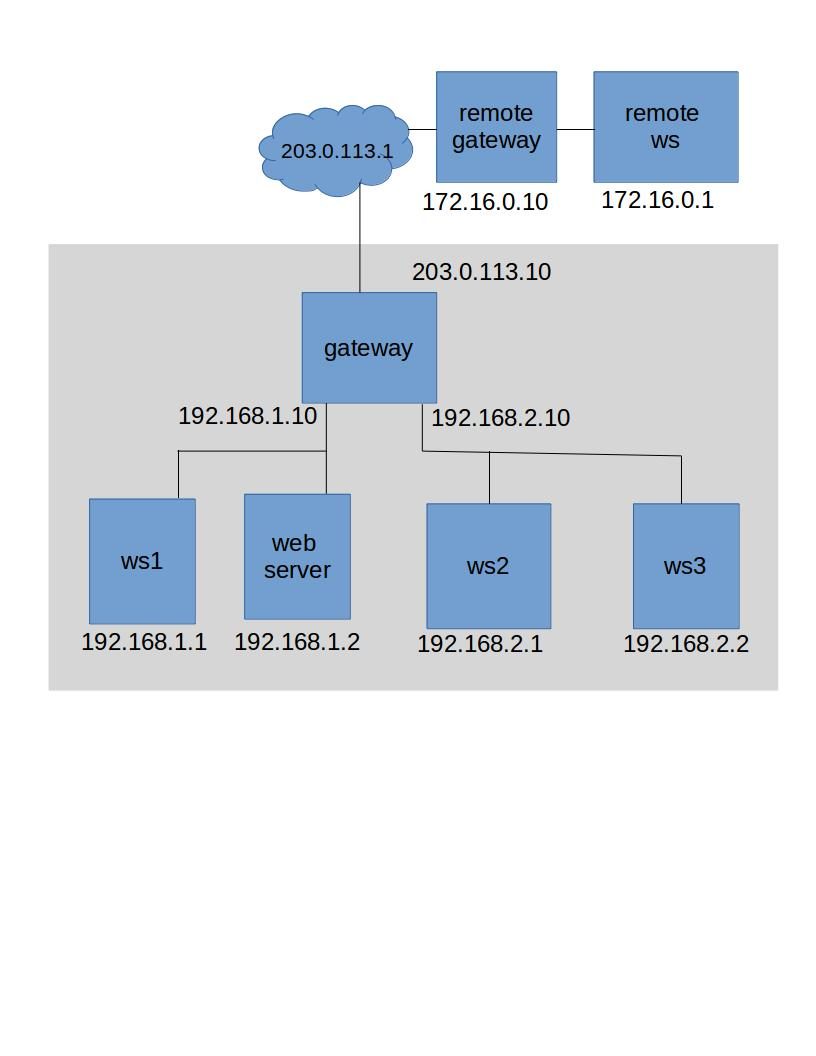
\includegraphics [width=0.8\textwidth]{snort.jpg}
\end{center}
\caption{Network topology for the snort lab}
\label{fig:topology}
\end{figure}

\section{Lab Tasks}
It is assumed that the student has received instruction or independent study on
the basic operation of Snort, and the general goals and mechanics of network intrusion detection.

Review the network topology.  In particular, consider the {\tt iptables} settings on the gateway.
These can be seen by reviewing the commands in {\tt /etc/rc.local}, which are used to
define the NAT translations and, critically for this lab, mirror traffic to the snort component. 

\subsection{Starting and stopping snort}
The Snort utility is installed on the snort component.  The home directory includes a {\tt start\_snort.sh}
script that will start the utility in \textit{Network Intrustion Dection Mode}, and display alerts
to the console.  For this lab, you are required to start snort with:
\begin{verbatim}
   ./start_snort.sh
\end{verbatim}
When it comes time to stop snort, e.g., to add rules, simply use {\tt CTL-C}.

\subsection{Pre-configured Snort rules}
The Snort utility includes a set of pre-configured rules that create alerts for known
suspicious network activity. The configuration on the snort component is largely as it
exists after initial installation of the snort utility.  To see an example of 
some of the preconfigured rules, perform an nmap scan of www.example.com from the remote
workstation:
\begin{verbatim}
    sudo nmap www.example.com
\end{verbatim}
\noindent Note the alerts displayed at the snort console.  The rules that generate these alerts can be seen,
along with all rules, in {\tt /etc/snort/rules/}

\subsection{Write a simple (bad) rule}
Custom rules are typically added to the file at {\tt /etc/snort/rules/local.rules}
Stop snort and add a rule that generates an alert for each packet within a TCP stream. For example:
\begin{verbatim}
alert tcp any any -> any any (msg:"TCP detected"; sid:00002;)
\end{verbatim}

\noindent That rule can be read as: ``Generate an alert whenever a TCP packet from any
address on any  port is sent to any address on any port, and include the message tagged as
{\tt msg:}, and give the rule an identifier of 00002.''
Then restart snort.  Test this rule by starting Firefox on the remote workstation:

\begin{verbatim}
    firefox www.example.com
\end{verbatim}

As you can see, the rule you wrote will overwhelm you with useless information.  So,
stop snort and delete the rule.

\subsection{Custom rule for CONFIDENTIAL traffic}
At the Firefox browser, which should be displaying the webpage from www.example.com,
we will display an unpublished web page that we know exists on the website.  In particular,
we have heard that the keen minds at the startup company have placed their confidential 
business plan at www.example.com/plan.html.  Take a look at it.

Now add a rule to your local.rules file on snort that will generate an alert 
whenever the text "CONFIDENTIAL" is sent out to the internet.  Reference 
the snort manual \url{https://www.snort.org/downloads/snortplus/snort_manual.pdf}
or existing rules to understand how to qualify alerts based on \textit{content}.  Be sure to include the
word "CONFIDENTIAL" in the alert message, and give the
rule its own unique sid.  After adding the rule, restart snort.

On the browser at the remote workstation, clear your history (Menu / Preferences 
Security \& Privacy), and then refresh the plan.html page.  You should see an alert at
the snort console.

\subsection{Effects of encryption}
Back at the Firefox browser, again clear the browser history. Now alter the URL to make
use of the web server SSL function.  Change the url to https://www.example.com/plan.html.
Do you see a new snort alert?  Why?

One solution to this problem is to use a reverse proxy in front of the web server.  This
reverse proxy would handle the incoming web traffic and manage the SSL connections.
The web server would then receive only clear-text HTTP traffic, and outgoing traffic from the web server
could then be mirrored to the IDS.  We will not pursue that solution in this lab.

\subsection{Watching internal traffic}
Go to the ws2 (mary) component and run nmap:
\begin{verbatim}
    sudo nmap www.example.com
\end{verbatim}
What do you see on the snort component?  Does it include the {\tt ICMP PING NMAP}
alert that you saw when the remote workstation ran nmap?  Why not?

Go to the gateway component and edit the {\tt /etc/rc.local} script so that traffic
from Mary's workstation is mirrored to the snort component.  You can do this by adding
this line to the section of that file that defines the packet mirroring:
\begin{verbatim}
   iptables -t mangle -A PREROUTING -i $lan2 -j TEE --gateway 192.168.3.1
\end{verbatim}

Then run the script to replace the {\tt iptables} rules with your new rules:
\begin{verbatim}
    sudo /etc/rc.local
\end{verbatim}
Now restart snort and again run nmap from mary's ws2 computer.


\subsection{Distinguishing traffic by address}
Start Firefox on mary's ws2 computer to view the confidential business plan:
\begin {verbatim}
    firefox www.example.com/plan.html
\end {verbatim}
Then observe the snort console.  This will not do!  The keen minds at the startup need to view their confidential
business plan without IDS alerts firing off.  But they do want to monitor
internal computers for suspicious traffic, e.g., nmap scans.  In this task, you 
will adjust your snort rule so that the CONFIDENTIAL alert only fires when the plan 
is accessed by addresses outside of
the site.  

If you review rules found in the {\tt/etc/snort/rules} directory, you will see that rules
have the general form of:
\begin{verbatim}
   alert <protocol> <source_addr> <src_port> ->  \
         <dest_addr> <dest_port> <rule options in parens>
\end{verbatim}

The snort rules include two address fields: {\tt source\_addr} and {\tt dest\_addr}. 
These addresses are used to check the
source from which the packet originated and the destination of the packet. The address
may be a single IP address or a network address. You likely have used the \textit{any} keyword to apply a
rule on all addresses. For network addresses, the address is followed by a slash character 
and number of bits in the netmask. For example, a network address of 192.168.2.0/24 
represents C class network 192.168.2.0 with 24 bits in the network mask.

Note that as a result of our use of NAT, all traffic from the web server destined for an
external address will have a destination address of the gateway, (i.e., 192.168.1.10), 
while web traffic destined for internal users will have destination addresses that match the internal user.

For this task, you must set your snort rules and traffic mirroring such that:
\begin{enumerate}
\item External access to the business plan generates an alert;
\item Internal access to the business plan does not generate an alert;
\item External or internal use of nmap will generate an ICMP NMAP PING alert.
\end{enumerate}
Your must test each of these criteria during a single snort session, i.e., if you change
a snort rule, or port mirroring, you must restart your tests.

\section{Submission}
After finishing the lab, go to the terminal on your Linux system that was used to start the lab and type:
\begin{verbatim}
    stoplab snort
\end{verbatim}
When you stop the lab, the system will display a path to the zipped lab results on your Linux system.  Provide that file to 
your instructor, e.g., via the Sakai site.

\end{document}
